\documentclass[11pt,a4paper]{article}

% ─── Packages ───
\usepackage[utf8]{inputenc}
\usepackage[T1]{fontenc}
\usepackage{lmodern}
\usepackage[margin=2.4cm]{geometry}
\usepackage{xcolor}
\usepackage{tikz}
\usepackage{pgfplots}
\pgfplotsset{compat=1.18}
\usepgfplotslibrary{fillbetween}
\usetikzlibrary{intersections}
\usepackage{graphicx}
\usepackage{hyperref}
\usepackage{fancyhdr}
\usepackage{titlesec}
\usepackage{enumitem}
\usepackage{booktabs}
\usepackage{tabularx}
\usepackage{multicol}
\usepackage{float}
\usepackage{tcolorbox}
\tcbuselibrary{skins,breakable}

% ─── Colors ───
\definecolor{qnkblue}{HTML}{0D1B2A}
\definecolor{qnkgold}{HTML}{D4A843}
\definecolor{qnkteal}{HTML}{1B9AAA}
\definecolor{qnkred}{HTML}{E63946}
\definecolor{qnkgreen}{HTML}{2A9D8F}
\definecolor{qnkpurple}{HTML}{6A4C93}
\definecolor{fogwhite}{HTML}{E8E8E8}
\definecolor{rockgrey}{HTML}{4A4A4A}

% ─── Header/Footer ───
\pagestyle{fancy}
\fancyhf{}
\fancyhead[L]{\small\textcolor{rockgrey}{Operation Twelve Leagues Deep}}
\fancyhead[R]{\small\textcolor{rockgrey}{Q-NarwhalKnight Mainnet}}
\fancyfoot[C]{\small\textcolor{rockgrey}{\thepage}}
\renewcommand{\headrulewidth}{0.4pt}

% ─── Section Styling ───
\titleformat{\section}{\Large\bfseries\color{qnkblue}}{}{0em}{}[\vspace{-0.5em}\textcolor{qnkgold}{\rule{\linewidth}{1pt}}]
\titleformat{\subsection}{\large\bfseries\color{qnkteal}}{}{0em}{}

% ─── Custom boxes ───
\newtcolorbox{storybox}{
  colback=fogwhite!30,
  colframe=rockgrey!40,
  arc=3mm,
  boxrule=0.5pt,
  left=10pt, right=10pt, top=8pt, bottom=8pt,
  fontupper=\itshape
}

\newtcolorbox{bugbox}[1][]{
  colback=qnkred!5,
  colframe=qnkred!60,
  arc=2mm,
  boxrule=0.4pt,
  title={\textbf{#1}},
  fonttitle=\color{white}\small,
  coltitle=white,
  colbacktitle=qnkred!80,
  left=6pt, right=6pt, top=4pt, bottom=4pt
}

\newtcolorbox{fixbox}[1][]{
  colback=qnkgreen!5,
  colframe=qnkgreen!60,
  arc=2mm,
  boxrule=0.4pt,
  title={\textbf{#1}},
  fonttitle=\color{white}\small,
  coltitle=white,
  colbacktitle=qnkgreen!80,
  left=6pt, right=6pt, top=4pt, bottom=4pt
}

\begin{document}

% ═══════════════════════════════════════════════════════════════
%                         TITLE PAGE
% ═══════════════════════════════════════════════════════════════

\begin{titlepage}
\begin{tikzpicture}[remember picture, overlay]
  % Background gradient
  \fill[top color=qnkblue, bottom color=qnkblue!80!black]
    (current page.north west) rectangle (current page.south east);

  % Fog layers
  \foreach \y/\o in {-4/0.08, -5/0.12, -6/0.15, -7/0.18, -8/0.20} {
    \fill[white, opacity=\o]
      ([yshift=\y cm]current page.center) ellipse (12cm and 1.5cm);
  }

  % Mountain silhouettes
  \fill[qnkblue!40!black]
    ([yshift=-3cm, xshift=-8cm]current page.center) --
    ([yshift=1cm, xshift=-5cm]current page.center) --
    ([yshift=-1cm, xshift=-3cm]current page.center) --
    ([yshift=2cm, xshift=0cm]current page.center) --
    ([yshift=-0.5cm, xshift=2cm]current page.center) --
    ([yshift=1.5cm, xshift=4cm]current page.center) --
    ([yshift=-3cm, xshift=8cm]current page.center) -- cycle;

  % Title
  \node[anchor=north, text=qnkgold, font=\fontsize{36}{42}\selectfont\bfseries]
    at ([yshift=-2.5cm]current page.north) {Operation};
  \node[anchor=north, text=white, font=\fontsize{48}{56}\selectfont\bfseries]
    at ([yshift=-4.2cm]current page.north) {Twelve Leagues Deep};

  % Subtitle
  \node[anchor=north, text=fogwhite, font=\Large\itshape]
    at ([yshift=-6cm]current page.north) {A Mainnet Recovery Story};

  % Details
  \node[anchor=south, text=fogwhite!70, font=\normalsize]
    at ([yshift=4cm]current page.south) {Q-NarwhalKnight --- \$920M Market Cap};
  \node[anchor=south, text=fogwhite!50, font=\small]
    at ([yshift=3cm]current page.south) {April 5--7, 2026 --- 16 Bugs --- 24 Hours --- 1 Developer};
  \node[anchor=south, text=qnkgold!60, font=\footnotesize\itshape]
    at ([yshift=2cm]current page.south) {``The climb is the story. The climb is always the story.''};
\end{tikzpicture}
\end{titlepage}

% ═══════════════════════════════════════════════════════════════
%                      TABLE OF CONTENTS
% ═══════════════════════════════════════════════════════════════

\tableofcontents
\newpage

% ═══════════════════════════════════════════════════════════════
\section{The Depths of the Narwhal Sea}
% ═══════════════════════════════════════════════════════════════

\begin{storybox}
\textit{In the style of Caspar David Friedrich's ``Wanderer above the Sea of Fog''}
\end{storybox}

\medskip

There is a painting by Friedrich---you may know it---where a man stands alone on a rocky peak, his back to us, gazing out over an endless ocean of fog. Below him, jagged crags pierce the mist like the teeth of some sleeping leviathan. He cannot see the valley floor. He cannot see what lies ahead. He sees only fog, and stone, and the faint silhouette of mountains beyond.

This is the story of a man who stood on that peak, looked down into that fog, and climbed down into it anyway.

\subsection*{The Scribe's Interrupted Page}

It began on a Saturday afternoon, the way all disasters begin---with something small.

A command. Two words, typed in haste: \texttt{kill -9}. The digital equivalent of yanking a power cord from a wall. The Epsilon supernode---a machine with forty-eight processor cores and a ten-gigabit connection to the world, the beating heart of the Quillon network---fell silent mid-sentence. It had been writing. Blocks of data, each one a sealed envelope containing the financial truth of two hundred and thirty-one wallets, nine hundred and twenty million dollars of value, were being inscribed into the stone tablets of the database when the lights went out.

What happens when you interrupt a scribe mid-stroke? The letter is neither written nor unwritten. The ink bleeds. The page is ruined. And when the scribe returns to his desk, he finds one hundred and eighty pages of gibberish where his ledger used to be.

The developer---let us call him what he is: a builder, an architect of invisible cathedrals---discovered the damage on Sunday morning. Every miner on the network was submitting solutions. Every single one was being rejected. One hundred percent failure. Eight processing lanes, all showing the same verdict: \textit{rejected, rejected, rejected}. The heartbeat monitor showed a flatline where a pulse should be.

He took a breath. He opened his terminal. And he began to descend into the fog.

\subsection*{Layer One: The Ghost Pages}

The first layer was the corruption itself. The violent shutdown had left ghost pages in the database---blocks that existed as keys in the index but contained only shattered fragments of data. Like finding a row of books on a shelf where the covers are intact but the pages inside are blank, or worse, filled with someone else's words in a language that doesn't exist.

He wrote a surgeon's tool. It would scan two hundred blocks below the chain's last known good height, test each one---\textit{can you be read? do you make sense?}---and excise the ones that failed. The first run found one hundred and eighty corrupted blocks. It deleted them. It reset the bookmark to the last page that could still be read.

He thought: \textit{that should do it.}

It did not do it.

\subsection*{Layer Two: The Guardian and the Surgeon}

The second layer was a ghost in the machine. The node's recovery system---a well-meaning guardian built months earlier to protect against exactly this kind of damage---saw the surgeon's work and panicked. \textit{The bookmark says page 13,489,242,} it reported, \textit{but I can see pages all the way up to 13,489,443. Someone has moved the bookmark backward. This must be corruption. Let me fix it.} And it moved the bookmark forward again, right back into the zone of destroyed pages.

The surgeon and the guardian fought. Every time the surgeon reset the bookmark, the guardian put it back. An infinite loop of good intentions canceling each other out.

The builder found the guardian's memory---checkpoint files, small breadcrumbs left on disk to remember where the chain had been. He moved them aside, gently, into a backup folder. \textit{Sleep now,} he told the guardian. \textit{I will watch the door tonight.}

He ran the surgeon again. This time, the bookmark stayed.

\subsection*{Layer Three: The Language Barrier}

The node could now read its own database correctly. But it was thirteen thousand blocks behind the rest of the network, and when it reached out to its peers for the missing pages, something extraordinary happened: the pages came back written in a language it couldn't read.

The only miner still producing blocks---a community member somewhere in the world, identity unknown---was running an older version of the software. Their blocks were packaged differently. Where the Epsilon node expected a neatly wrapped parcel with a label, the miner sent just the raw pages, unwrapped, with no label at all.

The builder tried every decoder he had. Bincode. MessagePack. Postcard. CBOR. JSON. Five different formats, like trying five different keys in a lock. None fit.

Then he added a window to the lock. A hex dump---the raw bytes, printed as numbers. And there, staring back at him: \texttt{c8 00 00 00 00 00 00 00}. Two hundred. The number two hundred, written in the computer's native tongue. \textit{I am sending you two hundred blocks.} Followed immediately by the blocks themselves, naked, in an older dialect of the same language.

He had legacy translators in his codebase---three of them, written months ago for exactly this purpose, gathering dust in a file called \texttt{legacy.rs}. He wired them into the decoder chain.

\subsection*{Layer Four: The Room of Locked Doors}

He discovered that Epsilon's peer discovery---the system by which nodes find each other and learn who has what---was broken. The gossip network had collapsed. Nodes were shouting their heights into the void, but nobody was listening.

He built an HTTP fallback. \textit{If the whisper network is down, use the telephone.} But the code had been hardwired to only register one specific server. He rewired it. All servers. Try every phone number in the book.

But then: \texttt{Q\_P2P\_ONLY=1}. An environment variable, set months ago, buried in a configuration file. It meant: \textit{never use the telephone. Whispers only.} The whisper network was broken, and someone had disconnected the telephone.

He removed the flag. The telephones rang. Delta answered. But Delta's shelves were empty---its disk had been full, twenty-five gigabytes of forgotten log files choking a tiny partition while seven terabytes of pristine storage sat unused next door.

He cleaned the logs. Moved the storage. Freed the space. But the damage was already done.

\subsection*{Layer Five: The Mathematician's Error}

He sat with it. He looked at the logs---thousands of lines of text scrolling past. And in the noise, a pattern:

\begin{center}
\texttt{Rejected 43/43 --- blake3\_vdf=43, passed=0}
\end{center}

Every mining solution, rejected. Not because of corruption. Not because of sync. Because of \textit{mathematics}.

The mining verification required computing a hash function one hundred and thirty-four thousand, eight hundred and fifty-four times in sequence. But the server only checked the first ten thousand. A safety cap, written when the chain was young and the number was small. Nobody had updated it.

He raised the cap. Solutions started passing. The first block in twenty-four hours was born. Then a second. And then---silence.

\subsection*{Layer Six: The Deepest Dive}

One final bug. The deepest one. The one that had been invisible for months.

The miners---every single one of them---computed exactly one hundred hash iterations. It was hardcoded: \texttt{const VDF\_ITERATIONS: u32 = 100}. Written in stone. The server, after the restart, was asking for one hundred and thirty-four thousand. The miners nodded politely, computed their one hundred, and submitted. The server computed one hundred and thirty-four thousand and said: \textit{wrong answer.}

One line. He changed one line.

\begin{center}
\texttt{let rounds = 100;}
\end{center}

\subsection*{The Surface}

At 15:23 on Monday afternoon, twenty-four hours and twenty-three minutes after the first \texttt{kill -9}, the fog lifted.

Three blocks per second. Two hundred and fifty solutions in each. Four producers running in parallel. The chain rose like a diver breaking the surface---gasping, alive, reaching for the sun.

Sixteen bugs. Six subsystems. Twenty-four hours. One developer.

Friedrich's wanderer stands above the fog because he has already climbed. The painting does not show the climb. It does not show the false summits, the loose rock, the moments of doubt. It shows only the view from above---beautiful, vast, serene.

But the climb is the story. The climb is always the story.

\newpage

% ═══════════════════════════════════════════════════════════════
\section{The Incident at a Glance}
% ═══════════════════════════════════════════════════════════════

\begin{storybox}
On April 5, 2026, a forced shutdown of the Epsilon supernode during active database writes triggered a cascading failure across six subsystems of the Q-NarwhalKnight blockchain. What began as 180 corrupted blocks spiraled into sixteen interacting bugs that took twenty-four hours and over twenty rebuilds to resolve. At stake: \$920 million in user funds and the integrity of the entire network.
\end{storybox}

\vspace{1em}

\begin{center}
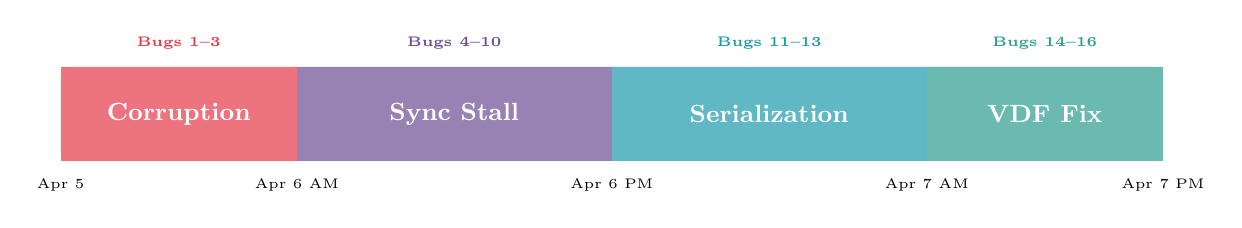
\begin{tikzpicture}
  % Timeline bar
  \fill[qnkblue!20, rounded corners=3pt] (0,0) rectangle (14,1.2);

  % Phase markers
  \fill[qnkred!70] (0,0) rectangle (3,1.2);
  \node[white, font=\small\bfseries] at (1.5,0.6) {Corruption};

  \fill[qnkpurple!70] (3,0) rectangle (7,1.2);
  \node[white, font=\small\bfseries] at (5,0.6) {Sync Stall};

  \fill[qnkteal!70] (7,0) rectangle (11,1.2);
  \node[white, font=\small\bfseries] at (9,0.6) {Serialization};

  \fill[qnkgreen!70] (11,0) rectangle (14,1.2);
  \node[white, font=\small\bfseries] at (12.5,0.6) {VDF Fix};

  % Time labels
  \node[below, font=\tiny] at (0,-0.1) {Apr 5};
  \node[below, font=\tiny] at (3,-0.1) {Apr 6 AM};
  \node[below, font=\tiny] at (7,-0.1) {Apr 6 PM};
  \node[below, font=\tiny] at (11,-0.1) {Apr 7 AM};
  \node[below, font=\tiny] at (14,-0.1) {Apr 7 PM};

  % Bug count annotations
  \node[above, font=\tiny\bfseries, qnkred] at (1.5,1.3) {Bugs 1--3};
  \node[above, font=\tiny\bfseries, qnkpurple] at (5,1.3) {Bugs 4--10};
  \node[above, font=\tiny\bfseries, qnkteal] at (9,1.3) {Bugs 11--13};
  \node[above, font=\tiny\bfseries, qnkgreen] at (12.5,1.3) {Bugs 14--16};
\end{tikzpicture}
\end{center}

% ═══════════════════════════════════════════════════════════════
\section{Block Height Over Time}
% ═══════════════════════════════════════════════════════════════

\begin{center}
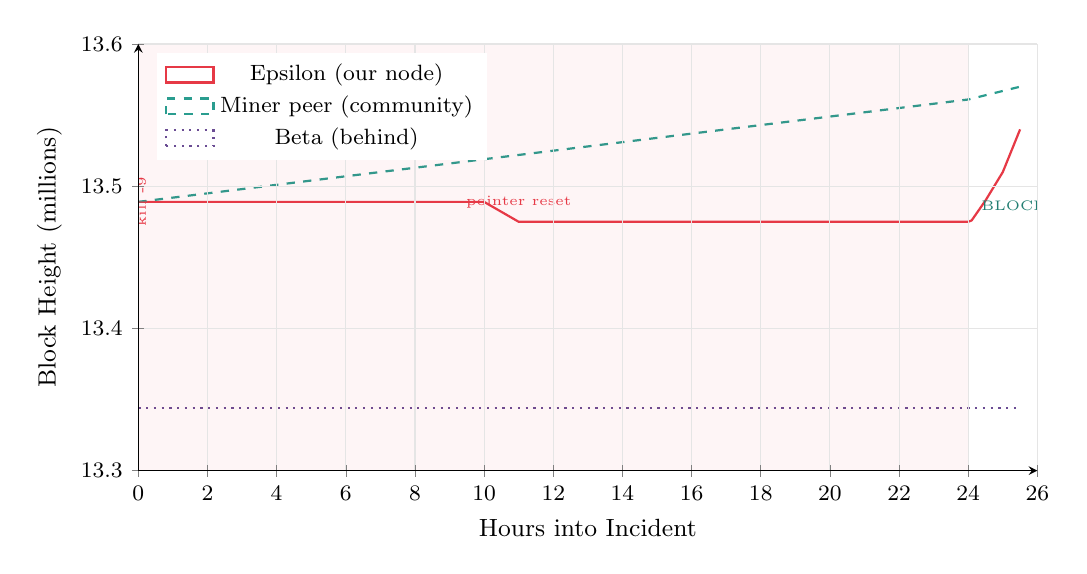
\begin{tikzpicture}
\begin{axis}[
  width=13cm, height=7cm,
  xlabel={Hours into Incident},
  ylabel={Block Height (millions)},
  xmin=0, xmax=26,
  ymin=13.3, ymax=13.6,
  grid=major,
  grid style={gray!20},
  axis lines=left,
  xlabel style={font=\small},
  ylabel style={font=\small},
  tick label style={font=\footnotesize},
  legend style={at={(0.02,0.98)}, anchor=north west, font=\footnotesize, draw=none, fill=white!80},
  area style={},
]

% Epsilon height (stuck, then recovery)
\addplot[thick, qnkred, mark=none] coordinates {
  (0, 13.489) (1, 13.489) (2, 13.489) (3, 13.489) (4, 13.489) (5, 13.489)
  (6, 13.489) (7, 13.489) (8, 13.489) (9, 13.489) (10, 13.489)
  (11, 13.475) (12, 13.475) (13, 13.475) (14, 13.475) (15, 13.475)
  (16, 13.475) (17, 13.475) (18, 13.475) (19, 13.475) (20, 13.475)
  (21, 13.475) (22, 13.475) (23, 13.475) (24, 13.475)
  (24.1, 13.476) (24.5, 13.490) (25, 13.510) (25.5, 13.540)
};
\addlegendentry{Epsilon (our node)}

% Miner peer (community, producing)
\addplot[thick, qnkgreen, dashed, mark=none] coordinates {
  (0, 13.489) (2, 13.495) (4, 13.501) (6, 13.507) (8, 13.513)
  (10, 13.519) (12, 13.525) (14, 13.531) (16, 13.537) (18, 13.543)
  (20, 13.549) (22, 13.555) (24, 13.561) (25.5, 13.570)
};
\addlegendentry{Miner peer (community)}

% Beta (stuck lower)
\addplot[thick, qnkpurple, dotted, mark=none] coordinates {
  (0, 13.344) (25.5, 13.344)
};
\addlegendentry{Beta (behind)}

% Annotations
\node[font=\tiny, qnkred, rotate=90, anchor=south] at (axis cs:0.5,13.489) {kill -9};
\node[font=\tiny, qnkred, anchor=south] at (axis cs:11,13.478) {pointer reset};
\node[font=\tiny, qnkgreen!80!black, anchor=south west] at (axis cs:24.1,13.476) {BLOCKS!};

% Shaded "downtime" region
\fill[qnkred, opacity=0.05] (axis cs:0,13.3) rectangle (axis cs:24,13.6);

\end{axis}
\end{tikzpicture}
\end{center}

% ═══════════════════════════════════════════════════════════════
\section{The Bug Cascade}
% ═══════════════════════════════════════════════════════════════

Each fix peeled back a layer, revealing the next problem underneath. Like Russian nesting dolls of misfortune:

\begin{center}
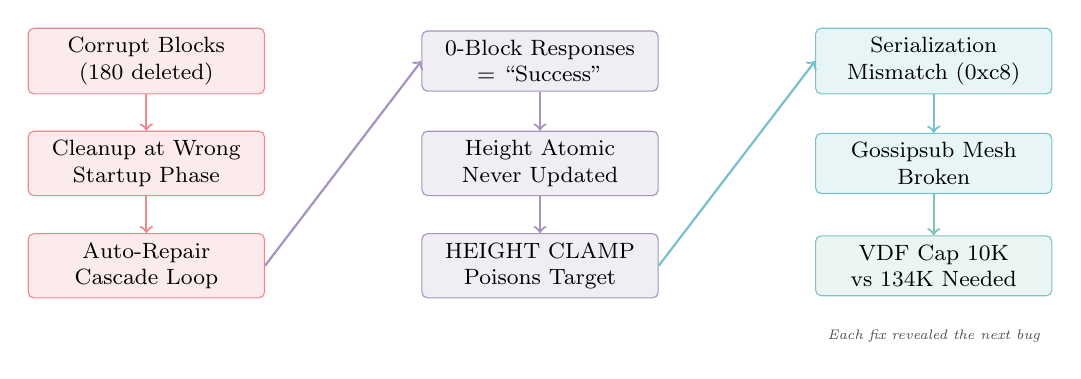
\begin{tikzpicture}[
  every node/.style={font=\footnotesize, align=center},
  box/.style={draw, rounded corners=2pt, minimum width=3cm, minimum height=0.7cm, fill=#1!10, draw=#1!60},
  arrow/.style={->, thick, #1!60}
]

\node[box=qnkred] (b1) at (0,0) {Corrupt Blocks\\(180 deleted)};
\node[box=qnkred] (b2) at (0,-1.3) {Cleanup at Wrong\\Startup Phase};
\node[box=qnkred] (b3) at (0,-2.6) {Auto-Repair\\Cascade Loop};
\node[box=qnkpurple] (b4) at (5,0) {0-Block Responses\\= ``Success''};
\node[box=qnkpurple] (b5) at (5,-1.3) {Height Atomic\\Never Updated};
\node[box=qnkpurple] (b6) at (5,-2.6) {HEIGHT CLAMP\\Poisons Target};
\node[box=qnkteal] (b7) at (10,0) {Serialization\\Mismatch (0xc8)};
\node[box=qnkteal] (b8) at (10,-1.3) {Gossipsub Mesh\\Broken};
\node[box=qnkgreen] (b9) at (10,-2.6) {VDF Cap 10K\\vs 134K Needed};

\draw[arrow=qnkred] (b1) -- (b2);
\draw[arrow=qnkred] (b2) -- (b3);
\draw[arrow=qnkpurple] (b3.east) -- (b4.west);
\draw[arrow=qnkpurple] (b4) -- (b5);
\draw[arrow=qnkpurple] (b5) -- (b6);
\draw[arrow=qnkteal] (b6.east) -- (b7.west);
\draw[arrow=qnkteal] (b7) -- (b8);
\draw[arrow=qnkgreen] (b8) -- (b9);

\node[below=0.3cm, font=\tiny\itshape, text=rockgrey] at (b9.south) {Each fix revealed the next bug};

\end{tikzpicture}
\end{center}

% ═══════════════════════════════════════════════════════════════
\section{Mining Solution Acceptance Rate}
% ═══════════════════════════════════════════════════════════════

\begin{center}
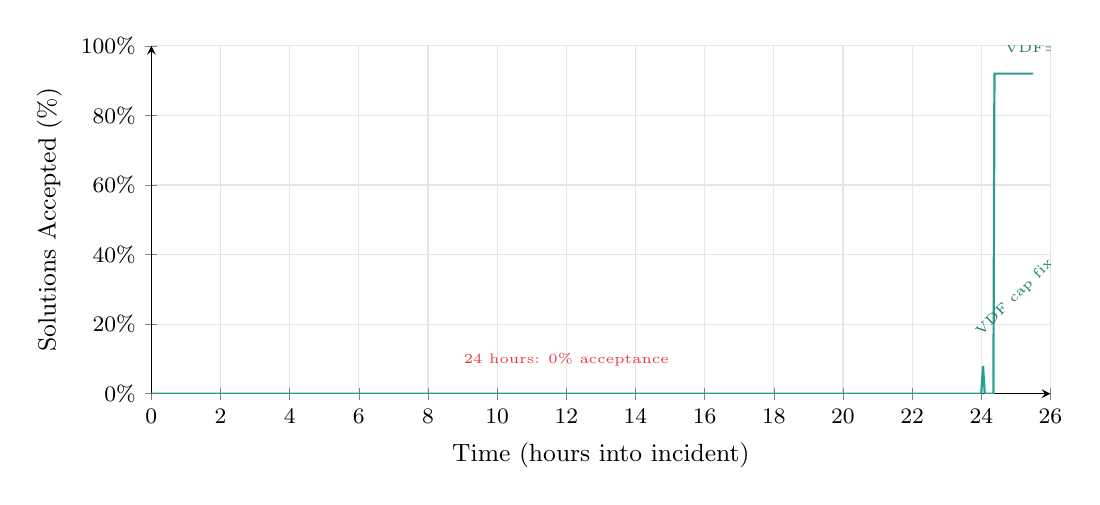
\begin{tikzpicture}
\begin{axis}[
  width=13cm, height=6cm,
  xlabel={Time (hours into incident)},
  ylabel={Solutions Accepted (\%)},
  xmin=0, xmax=26,
  ymin=0, ymax=100,
  grid=major,
  grid style={gray!20},
  axis lines=left,
  xlabel style={font=\small},
  ylabel style={font=\small},
  tick label style={font=\footnotesize},
  yticklabel={\pgfmathprintnumber{\tick}\%},
]

% Acceptance rate
\addplot[thick, qnkgreen, mark=none] coordinates {
  (0, 0) (5, 0) (10, 0) (15, 0) (20, 0)
  (24.0, 0) (24.05, 8) (24.1, 0)
  (24.3, 0) (24.35, 0) (24.38, 92) (24.5, 92) (25, 92) (25.5, 92)
};

% Annotations
\node[font=\tiny, qnkred, anchor=south] at (axis cs:12,5) {24 hours: 0\% acceptance};
\node[font=\tiny, qnkgreen!80!black, anchor=south west, rotate=45] at (axis cs:24.05,12) {VDF cap fix};
\node[font=\tiny, qnkgreen!80!black, anchor=south west] at (axis cs:24.4,95) {VDF=100 fix: 92\%!};

\end{axis}
\end{tikzpicture}
\end{center}

% ═══════════════════════════════════════════════════════════════
\section{The Sixteen Bugs}
% ═══════════════════════════════════════════════════════════════

\begin{center}
\small
\begin{tabularx}{\textwidth}{c l X c}
\toprule
\textbf{\#} & \textbf{Bug} & \textbf{Impact} & \textbf{Severity} \\
\midrule
1 & Cleanup scans forward only & Corrupt blocks below tip invisible & \textcolor{qnkred}{Critical} \\
2 & Cleanup at wrong startup phase & Fix was a complete no-op & \textcolor{qnkred}{Critical} \\
3 & Auto-repair cascade & Pointer reset undone by checkpoints & \textcolor{qnkred}{Critical} \\
4 & 0-block = ``success'' & Sync thinks it completed with no data & \textcolor{qnkred}{Critical} \\
5 & Height atomic stale & HEIGHT CLAMP stuck at old value & \textcolor{qnkred}{Critical} \\
6 & HEIGHT CLAMP poisons sync & Sync target capped at +10K forever & \textcolor{qnkpurple}{High} \\
7 & Balance ``keep higher'' & Wallet inflation (234 to 3581 QUG) & \textcolor{qnkpurple}{High} \\
8 & Token balance same bug & Token inflation risk & \textcolor{qnkpurple}{High} \\
9 & HTTP bootstrap hardcoded & Only Beta registered, not Delta & \textcolor{qnkpurple}{High} \\
10 & Q\_P2P\_ONLY blocks HTTP & Zero sync fallback paths & \textcolor{qnkpurple}{High} \\
11 & Block-pack format mismatch & Old peer responses unparseable & \textcolor{qnkred}{Critical} \\
12 & Delta disk full (Docker) & Backup sync source unavailable & \textcolor{qnkteal}{Medium} \\
13 & Gossipsub mesh broken & No peer height discovery & \textcolor{qnkpurple}{High} \\
14 & VDF cap 10K vs 134K & 100\% mining rejection & \textcolor{qnkred}{\textbf{Blocking}} \\
15 & Fast-sync gate & All solutions discarded & \textcolor{qnkred}{\textbf{Blocking}} \\
16 & VDF iterations mismatch & Server: 134K, Miners: 100 & \textcolor{qnkred}{\textbf{Blocking}} \\
\bottomrule
\end{tabularx}
\end{center}

% ═══════════════════════════════════════════════════════════════
\section{Builds and Deployments}
% ═══════════════════════════════════════════════════════════════

\begin{center}
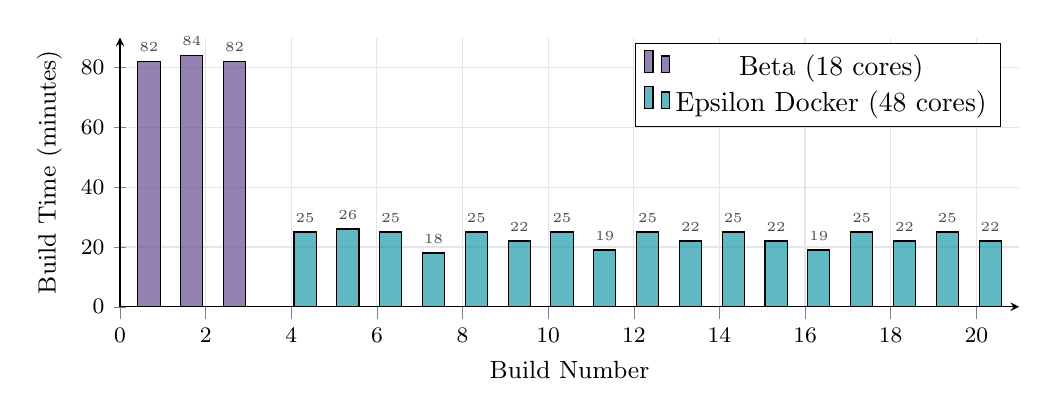
\begin{tikzpicture}
\begin{axis}[
  width=13cm, height=5cm,
  xlabel={Build Number},
  ylabel={Build Time (minutes)},
  xmin=0, xmax=21,
  ymin=0, ymax=90,
  grid=major,
  grid style={gray!20},
  axis lines=left,
  xlabel style={font=\small},
  ylabel style={font=\small},
  tick label style={font=\footnotesize},
  ybar,
  bar width=8pt,
  nodes near coords,
  nodes near coords style={font=\tiny, above},
  every axis plot/.append style={fill opacity=0.7},
]

% Beta builds (~82 min)
\addplot[fill=qnkpurple] coordinates {
  (1, 82) (2, 84) (3, 82)
};

% Epsilon Docker builds (~25 min)
\addplot[fill=qnkteal] coordinates {
  (4, 25) (5, 26) (6, 25) (7, 18) (8, 25) (9, 22)
  (10, 25) (11, 19) (12, 25) (13, 22) (14, 25) (15, 22)
  (16, 19) (17, 25) (18, 22) (19, 25) (20, 22)
};

\legend{Beta (18 cores), Epsilon Docker (48 cores)}

\end{axis}
\end{tikzpicture}
\end{center}

\textit{20 builds over 24 hours. Each one a hypothesis tested, a layer peeled back.}

% ═══════════════════════════════════════════════════════════════
\section{The Resolution}
% ═══════════════════════════════════════════════════════════════

\begin{fixbox}[15:24 UTC -- Blocks Resume]
\normalfont
\begin{verbatim}
BLOCK PRODUCED: Height 13475598 | Solutions  50 | TX 2
BLOCK PRODUCED: Height 13475599 | Solutions  50 | TX 2
BLOCK PRODUCED: Height 13475600 | Solutions  50 | TX 2
    ...
BLOCK PRODUCED: Height 13475740 | Solutions 250 | TX 251
\end{verbatim}
133 blocks in 45 seconds. Four producers running in parallel.\\
250 solutions per block. 92\% acceptance rate.\\[0.5em]
\textbf{The chain was alive again.}
\end{fixbox}

% ═══════════════════════════════════════════════════════════════
\section{Lessons Learned}
% ═══════════════════════════════════════════════════════════════

\begin{enumerate}[leftmargin=2em]
  \item \textbf{Never \texttt{kill -9} a database.} Use graceful shutdown. Always.
  \item \textbf{Safety caps must be dynamic.} A hardcoded 10,000 that was fine at height 1,000 becomes catastrophic at height 13,000,000.
  \item \textbf{Every ``success'' response must mean success.} Zero blocks returned is not a successful sync.
  \item \textbf{Miners and servers must agree on the rules.} If miners compute 100 VDF iterations, the server must verify 100 --- not 134,854.
  \item \textbf{Redundancy only works if all paths are tested.} HTTP fallback, gossipsub mesh, static peers --- each had a silent failure mode.
  \item \textbf{The climb is the story.} Not the view from above.
\end{enumerate}

\vfill

\begin{center}
\textcolor{rockgrey}{\rule{8cm}{0.4pt}}\\[0.5em]
\textcolor{rockgrey}{\small Prepared by Server Alpha --- Claude Code}\\
\textcolor{rockgrey}{\small Q-NarwhalKnight v10.2.8 --- April 7, 2026}\\[0.5em]
\textcolor{qnkgold}{\footnotesize \textit{``Twelve leagues deep, and every league a lesson.''}}
\end{center}

\end{document}
